
\chapter{\myenchttl{Programming with Karel the Robot}}
%https://tex.stackexchange.com/questions/10555/hyperref-warning-token-not-allowed-in-a-pdf-string
\XeTeXlinebreaklocale "my_MM"  %Myanmar line and character breaks
\XeTeXinterwordspaceshaping=2
\begin{sloppypar}



\enprogramming\ ဆိုတာဘာလဲရှင်းပြဖို့ စာတွေအများကြီးရေးနေတာထက် လက်တွေ့ \enprogram လေးတွေ စရေးကြည့်ပြီးမှ \mmprogramming ဆိုတာ ဘာလဲ ပြောပြလိုက်ရင် ပိုပြီးနားလည် သဘောပေါက်လွယ်တယ်။ 

\begin{figure}[h]
    \caption{ကားရဲလ်နှင့်  ကားရဲလ်၏ကမ္ဘာ}\label{fig:meet_karel}
    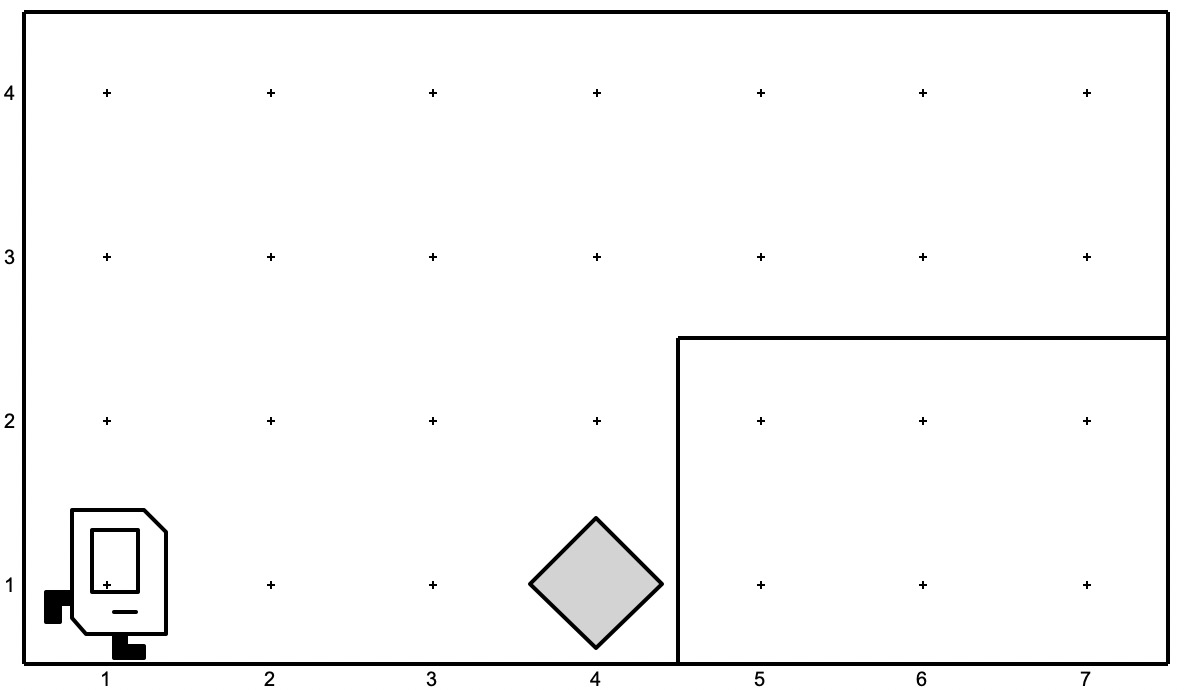
\includegraphics[width=4in, left]{ch01/meet_karel.jpg}
\end{figure}

\begin{figure}[tbh!]
    \caption{\mmbeeper နေရာရွှေ့ပြီး}\label{fig:meet_karel_aft}
    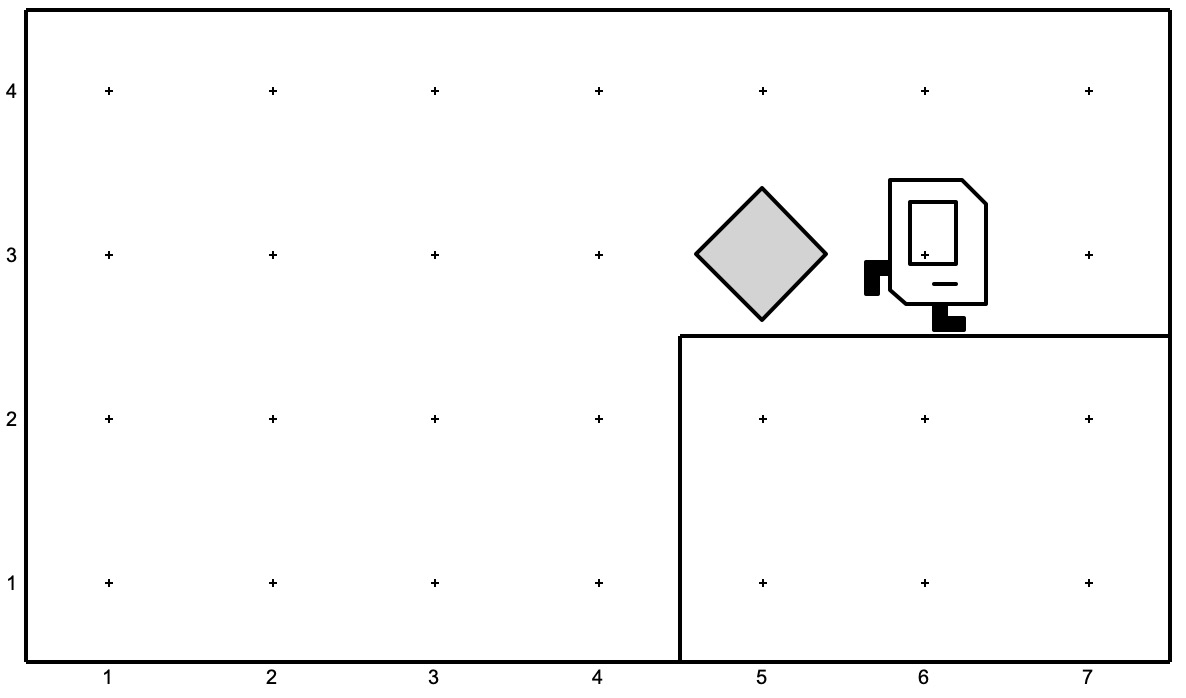
\includegraphics[width=4in, left]{ch01/meet_karel_aft.jpg}
\end{figure}

\section{ကားရဲလ်နှင့် မိတ်ဆက်ခြင်း}
ဒါ့ကြောင့် စက်ရုပ်ကားရဲလ်\myen{(Karel the Robot)}ကို သူရောက်နေတဲ့ ကမ္ဘာမှာ အလုပ်တွေ လုပ်ခိုင်းဖို့ \mmprogram လေးတွေ  အရင်ဆုံး ရေးကြည့်ကြမယ်။ \Fig \vref*{fig:meet_karel} မှာ ပြထားတာက ကားရဲလ် ရောက်ရှိနေမယ့် နမူနာ ကမ္ဘာပါ။ ကားရဲလ်ရဲ့ ကမ္ဘာထဲက မီးခိုးရောင် ဆနွင်းမကင်းကွက်ပုံ အရာကို \enbeeper\ လို့ ခေါ်တယ်။ 

 ကားရဲလ်က စကားပြောပြီး ခိုင်းလို့မရဘူး။ သူနားလည်တဲ့ \encommand တွေကို \mmprogram ရေးပြီးပဲ ခိုင်းလို့ရတယ်။ 

\section{ကားရဲလ်နားလည်သော \mmcommand လေးခု}
ကားရဲလ်က အခြေခံအားဖြင့် \mmcommand လေးခုကိုပဲ နားလည်တယ်။ \mycode{move, turnLeft, putBeeper, pickBeeper} \mmcommand တို့ ဖြစ်တယ်။ \mycode{move} ကွန်မန်းက သူရပ်နေတဲ့ \mmcorner ကနေ ရှေ့တည့်တည့် ကပ်ရပ် \mmcorner ကို ရွှေ့ခိုင်းတာ။ \mmcorner ‌တွေကို အပေါင်းသင်္ကေတ လေးတွေနဲ့ ပြထားတယ်။ ပုံထဲမှာ သေးနေတဲ့အတွက် အစက်လေးတွေလို့ ထင်ရတယ်။ 

ကားရဲလ်ကို \mycode{putBeeper} ကွန်မန်းပေးလိုက်ရင်တော့ ကားရဲလ်က သူရှိနေတဲ့ ကွန်နာမှာ ဘိပါ\myen{(beeper)} လို့ခေါ်တဲ့ အတုံးလေး တစ်ခုချထားလိမ့်မယ်။ 

\mycode{pickBeeper} ကွန်မန်းက ဘိပါကောက်ခိုင်းတာပါ။ ကားရဲလ်ရောက်နေတဲ့ ကွန်နာမှာ ဘိပါရှိရင် ဒီကွန်မန်းနဲ့ ကောက်ခိုင်းလို့ရတယ်။ 

\begin{figure}[tbh!]
    \begin{subfigure}[t]{0.46\textwidth}
        \adjincludegraphics[height=1.18in,trim={0 0 {.44\width} {.55\height}}, clip, left]{ch01/bef_move.jpg}
        \caption{ကနဦး အနေအထား}
    \end{subfigure}
    \hspace{0.1in}
    \begin{subfigure}[t]{0.46\textwidth}
        \adjincludegraphics[height=1.18in,trim={0 0 {.44\width} {.55\height}}, clip, left]{ch01/aft_1st_move.jpg}
        \caption{\myttlcode{move} \mmcommand လုပ်ဆောင်ပြီး}
    \end{subfigure}

    \begin{subfigure}[t]{0.46\textwidth}
        \adjincludegraphics[height=1.18in,trim={0 0 {.44\width} {.55\height}}, clip, left]{ch01/aft_2nd_move.jpg}
        \caption{\myttlcode{move} \mmcommand တစ်ခါထပ်၍ လုပ်ဆောင်ပြီး}
    \end{subfigure}
    \hspace{0.12in}
    \begin{subfigure}[t]{0.46\textwidth}
        \adjincludegraphics[height=1.18in,trim={0 0 {.44\width} {.55\height}}, clip, left]{ch01/aft_pick.jpg}
        \caption{\myttlcode{pickBeeper} \mmcommand လုပ်ဆောင်ပြီး}
    \end{subfigure}

    \begin{subfigure}[t]{0.46\textwidth}
        \adjincludegraphics[height=1.18in,trim={0 0 {.44\width} {.55\height}}, clip, left]{ch01/aft_3rd_move.jpg}
        \caption{\myttlcode{move} \mmcommand တစ်ခါထပ်၍ လုပ်ဆောင်ပြီး}
    \end{subfigure}
    \hspace{0.1in}
    \begin{subfigure}[t]{0.46\textwidth}
        \adjincludegraphics[height=1.18in,trim={0 0 {.44\width} {.55\height}}, clip, left]{ch01/aft_put.jpg}
        \caption{\myttlcode{putBeeper} \mmcommand လုပ်ဆောင်ပြီး}        
    \end{subfigure}

    \caption{\myttlcode{move, pickBeeper, putBeeper} \mmcommand အသီးသီး အလုပ်လုပ်ပုံ}
    \label{fig:bef_and_after_commands}
\end{figure}

\mycode{turnLeft} ကွန်မန်းကတော့  ဘယ်ဘက်လှည့်ခိုင်းတာ။ မူလအနေအထားကနေ \mycode{turnLeft} ကွန်မန်းပေးလိုက်တဲ့ အခါမှာ မျက်နှာမူရာ အရပ် ပြောင်းသွားပုံကို \Fig \vref*{fig:bef_and_after_turnLeft} တွင်ကြည့်ပါ။ ညာဘက်လှည့်ခိုင်းဖို့ ကားရဲလ်ကိို \mycode{turnRight} \mmcommand နဲ့တော့ ခိုင်းလို့မရဘူး။ သူက \mycode{turnRight}  \mmcommand ကို နားမလည်ပါဘူး။

\begin{figure}[tbh!]
    \begin{subfigure}[t]{0.4\textwidth}
        
\includegraphics[scale=0.2, left]{ch01/karel_icon_E.png}
        \caption{မူလ အနေအထား(အရှေ့ဘက်လှည့်)}    
    \end{subfigure}
    \begin{subfigure}[t]{0.4\textwidth}
        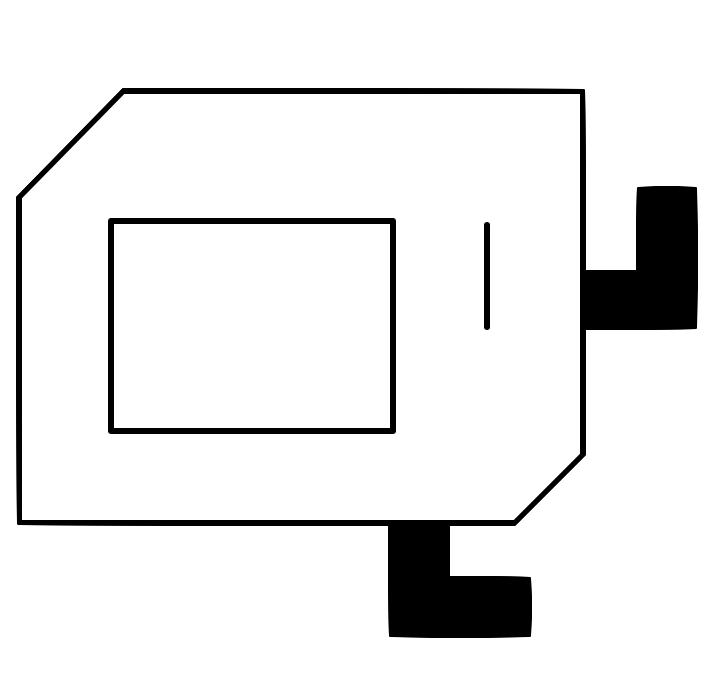
\includegraphics[scale=0.2, left]{ch01/karel_icon_N.png}
        \caption{\myttlcode{turnLeft} တစ်ကြိမ်လုပ်ဆောင်ပြီး}
    \end{subfigure}
    \begin{subfigure}[t]{0.4\textwidth}
        
\includegraphics[scale=0.2, left]{ch01/karel_icon_W.png}
        \caption{\myttlcode{turnLeft} တစ်ကြိမ် ထပ်၍လုပ်ဆောင်ပြီး}
    \end{subfigure}
    \begin{subfigure}[t]{0.4\textwidth}
        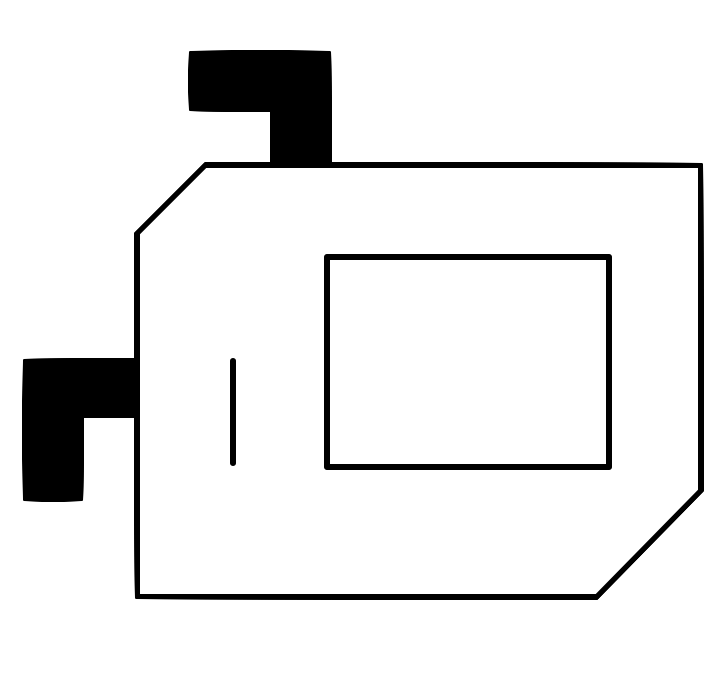
\includegraphics[scale=0.2, left]{ch01/karel_icon_S.png}
        \caption{\myttlcode{turnLeft} တစ်ကြိမ် ထပ်၍လုပ်ဆောင်ပြီး}
    \end{subfigure}
    \begin{subfigure}[t]{0.4\textwidth}
        
\includegraphics[scale=0.2, left]{ch01/karel_icon_E.png}
        \caption{\myttlcode{turnLeft} နောက်ဆုံးတစ်ကြိမ် လုပ်ဆောင်ပြီး}
    \end{subfigure}
    \caption{ကနဦး အရှေ့ဘက် မျက်နှာမူနေရာမှ}
    \label{fig:bef_and_after_turnLeft}
\end{figure}

\section{\mymmchsec{}{ပထမဆုံး ကားရဲလ်} \mmprogram}
\enbeeper ကို မူလနေရာကနေ \Fig \vref*{fig:meet_karel_aft} မှာပြထားတဲ့ နေရာကို ရွှေ့ခိုင်းရမှာပါ။ \mmcommand တွေကို ဘယ်လို အစဉ်အတိုင်းပေးရမလဲ။ \mmbeeper ရှိတဲ့နေရာကိုသွားပြီး \mmbeeper ကောင်ခိုင်းဖို့က \mycode{move, move, move, pickBeeper} \mmcommand ပေးမယ်။ ပြီးတဲ့အခါ ရှေ့မှာနံရံရှိနေတယ်။ ဆက်သွားလို့မရတော့ဘူး။ မြောက်ဘက်ကို သွားခိုင်းဖို့ \mycode{turnLeft}။ နှစ်ကြိမ်ထပ်ပြီးရွှေ့ခိုင်းရမယ်ဆိုတော့ \mycode{move, move}။ အရှေ့ဘက် ပြန်လှည့်ခိုင်းဖို့ ညာဘက်လှည့်ခိုင်းရမယ်။ ဒါပေမယ့် \mycode{turnRight} \mmcommand မရှိဘူး။ \mycode{turnLeft} သုံးခါလုပ်ခိုင်းလိုက်ရင်လည်း အရှေ့ဘက်လှည့်သွားမှာပဲ။ တစ်ခါထပ်ပြီး \mycode{move} ခိုင်းလိုက်ရင် \mmbeeper ကိုထားခိုင်းချင်တဲ့နေရာ ရောက်ပြီ။ \mycode{putBeeper} နဲ့ \mmbeeper ချထားခိုင်းလိုက်မယ်။ \mmbeeper ကိုမြင်သာအောင် \mycode{move} တစ်ခါ ထပ်လုပ်ခိုင်းလိုက်မယ်။

အစဉ်အတိုင်း ပေးရမယ့် \mmcommand တွေက \mycode{move, move, move, pickBeeper, turnLeft, move, move, turnLeft, turnLeft, turnLeft, move, putBeeper, move} ဖြစ်မယ်။ ဒီအစီအစဉ်အတိုင်း \mmcommand တွေကို \mmprogram ရေးပေးရမယ်။ \enJPL ကို အသုံးပြုပြီး ရေးရမှာပါ။ 

\mmprogram ရေးဖို့အတွက် \encomputer\ နားလည်တဲ့ ဘာသာစကား တစ်မျိုးမျိုးကို အသုံးပြုပြီး ရေးရတယ်။ \mmcomputer\ နားလည်တဲ့၊ \mmcomputer ပရိုဂရမ်ရေးဖို့ အသုံးပြုတဲ့ ဘာသာစကားကို \enPL\ လို့ ခေါ်တယ်။ 

မြန်မာ၊ အင်္ဂလိပ် စသည်ဖြင့် လူတွေရဲ့ ဘာသာစကားတွေမှာ သဒ္ဒါရှိသလိုပဲ \mmPL တွေမှာလည်း သဒ္ဒါရှိတယ်။ \mmprogram ရေးတဲ့အခါ အသုံးပြုတဲ့ \mmPL ရဲ့ ရေးပုံရေးနည်း၊ စည်းမျဉ်းစည်းကမ်း သတ်မှတ်ချက်တွေကို လိုက်နာဖို့လိုတယ်။ \mmPL ရဲ့ သဒ္ဒါကို \ensyntax\ လို့ ခေါ်တယ်။

ဒီအခန်းအတွက်က \mmsyntax အသေးစိတ် နားလည်ဖို့ မလိုသေးဘူး။ \enJPL ရဲ့ လိုအပ်ချက်အရ ပုံစံချပေးထားတဲ့ ကားရဲလ် \mmprogram\ \entemplate ကိုအသုံးပြုပြီး \mmcommand တွေကို \entemplate ထဲမှာပဲဖြည့်ရေးမယ်။ \entemplate က အခုလိုပုံစံပါ။

\begin{lstcodesimple}[float, caption=ကားရဲလ် ပရိုဂရမ် template]
public class ClassName extends stanford.karel.Karel{ 
        public void run(){
                //Karel commands
        }        
}
\end{lstcodesimple}




\section{IntelliJ}
\mmprogram\ ‌ရေးဖို့ \enintellij \enIDE ကို ဖွင့်။


\subsection{\myttlcode{class} သတ်မှတ်ခြင်း}
\mycode{class} တစ်ခုသတ်မှတ်ဖို့အတွက် 

\begin{lstcodesimple}[caption=\myttlcode{class} သတ်မှတ်သည့် ဆင်းတက်စ်]
    public class MeetKarel extends stanford.karel.Karel{
            
    }
\end{lstcodesimple}

\subsection{\myttlcode{class} သတ်မှတ်ခြင်း}
\mycode{class} တစ်ခုသတ်မှတ်ဖို့အတွက် 

\begin{lstcodesimple}[caption=\myttlcode{class} သတ်မှတ်သည့် ဆင်းတက်စ်]
    public class MeetKarel extends stanford.karel.Karel{
            
    }
\end{lstcodesimple}

\section{Karel's World}
\Fig \vref*{fig:meet_karel} 
အနောက်မှအရှေ့ \mmcorner တွေ တလျှောက်က \enstreet တွေ ဖြစ်ပြီး တောင်မှမြောက် \mmcorner တွေ တလျှောက်က \enavenue တွေ ဖြစ်တယ်။ 

\mmcorner တွေက \mmavenue နဲ့ \mmstreet တွေဆုံတဲ့ လမ်းဆုံတွေ ဖြစ်တယ်။ \mmcorner တစ်ခုကို ရည်ညွှန်းဖို့ \mmavenue နဲ့ \mmstreet နံပါတ်‌တွေကို အသုံးပြုမယ်။ ကားရဲလ်က (၁,၁) \mmcorner၊ \mmbeeper က (၃,၁) \mmcorner မှာရှိနေတယ်။ ပထမ‌‌နံပါတ်က \mmavenue ၊ ဒုတိယက \mmstreet နံပါတ်ပါ။ “\mmbeeper က (၃,၁) \mmcorner မှာရှိတယ်”  လို့ရေးရင် \mmbeeper က နံပါတ် ၃ \mmavenue\ နဲ့ ၁ \mmstreet ဆုံတဲ့ \mmcorner မှာ ရှိနေတယ်လို့ ဆိုလိုတာ။



\section{ကားရဲလ် ပရိုဂရမ်ကို ခွဲခြမ်းစိတ်ဖြာကြည့်ခြင်း}

\begin{lstcodesimple}[language = Java, float=ht]
    class ClassName {
            
    }
\end{lstcodesimple}

\begin{lstcodesimple}[language = Java, float]
    public class MeetKarel{
            
    }
\end{lstcodesimple}

\begin{lstcodesimple}[language = Java, float=hb]
    public class MeetKarel extends stanford.karel.Karel{
            
    }
\end{lstcodesimple}

\begin{lstcodesimple}[language = Java, float]
    import stanford.karel.Karel;
    public class MeetKarel extends {
            
    }
\end{lstcodesimple}

\begin{lstcodesimple}[language = Java, float]
    public class MeetKarel extends stanford.karel.Karel{
            public void run(){

            }            
    }
\end{lstcodesimple}

\end{sloppypar}
